% 图 78.2 —— 由 `checks/emit_hand.py` 自动拼出（probe 精测 + prims2 图元分解）
%%
% ⚠ 这是**稿子不是成品**：跑 `checks/checkhand.py 78.2` 看指标 + 看叠合图。
%%
%% ⚠ 待核：
%   · 本图 probe 报出阴影族 1 个 —— **本脚本不生成阴影**（要照原书手写）；prims2 的 strokes 里可能含阴影线，核对时留意别画重
%   · 可疑字形 1 项（空心圈 ⊙ 常被认成字母 o）—— 见文件末
%%
\documentclass[12pt]{standalone}
\usepackage{fontspec}
\setsansfont{Arial}
\newfontfamily\mfallback{DejaVu Sans}
\usepackage{tikz}
\begin{document}
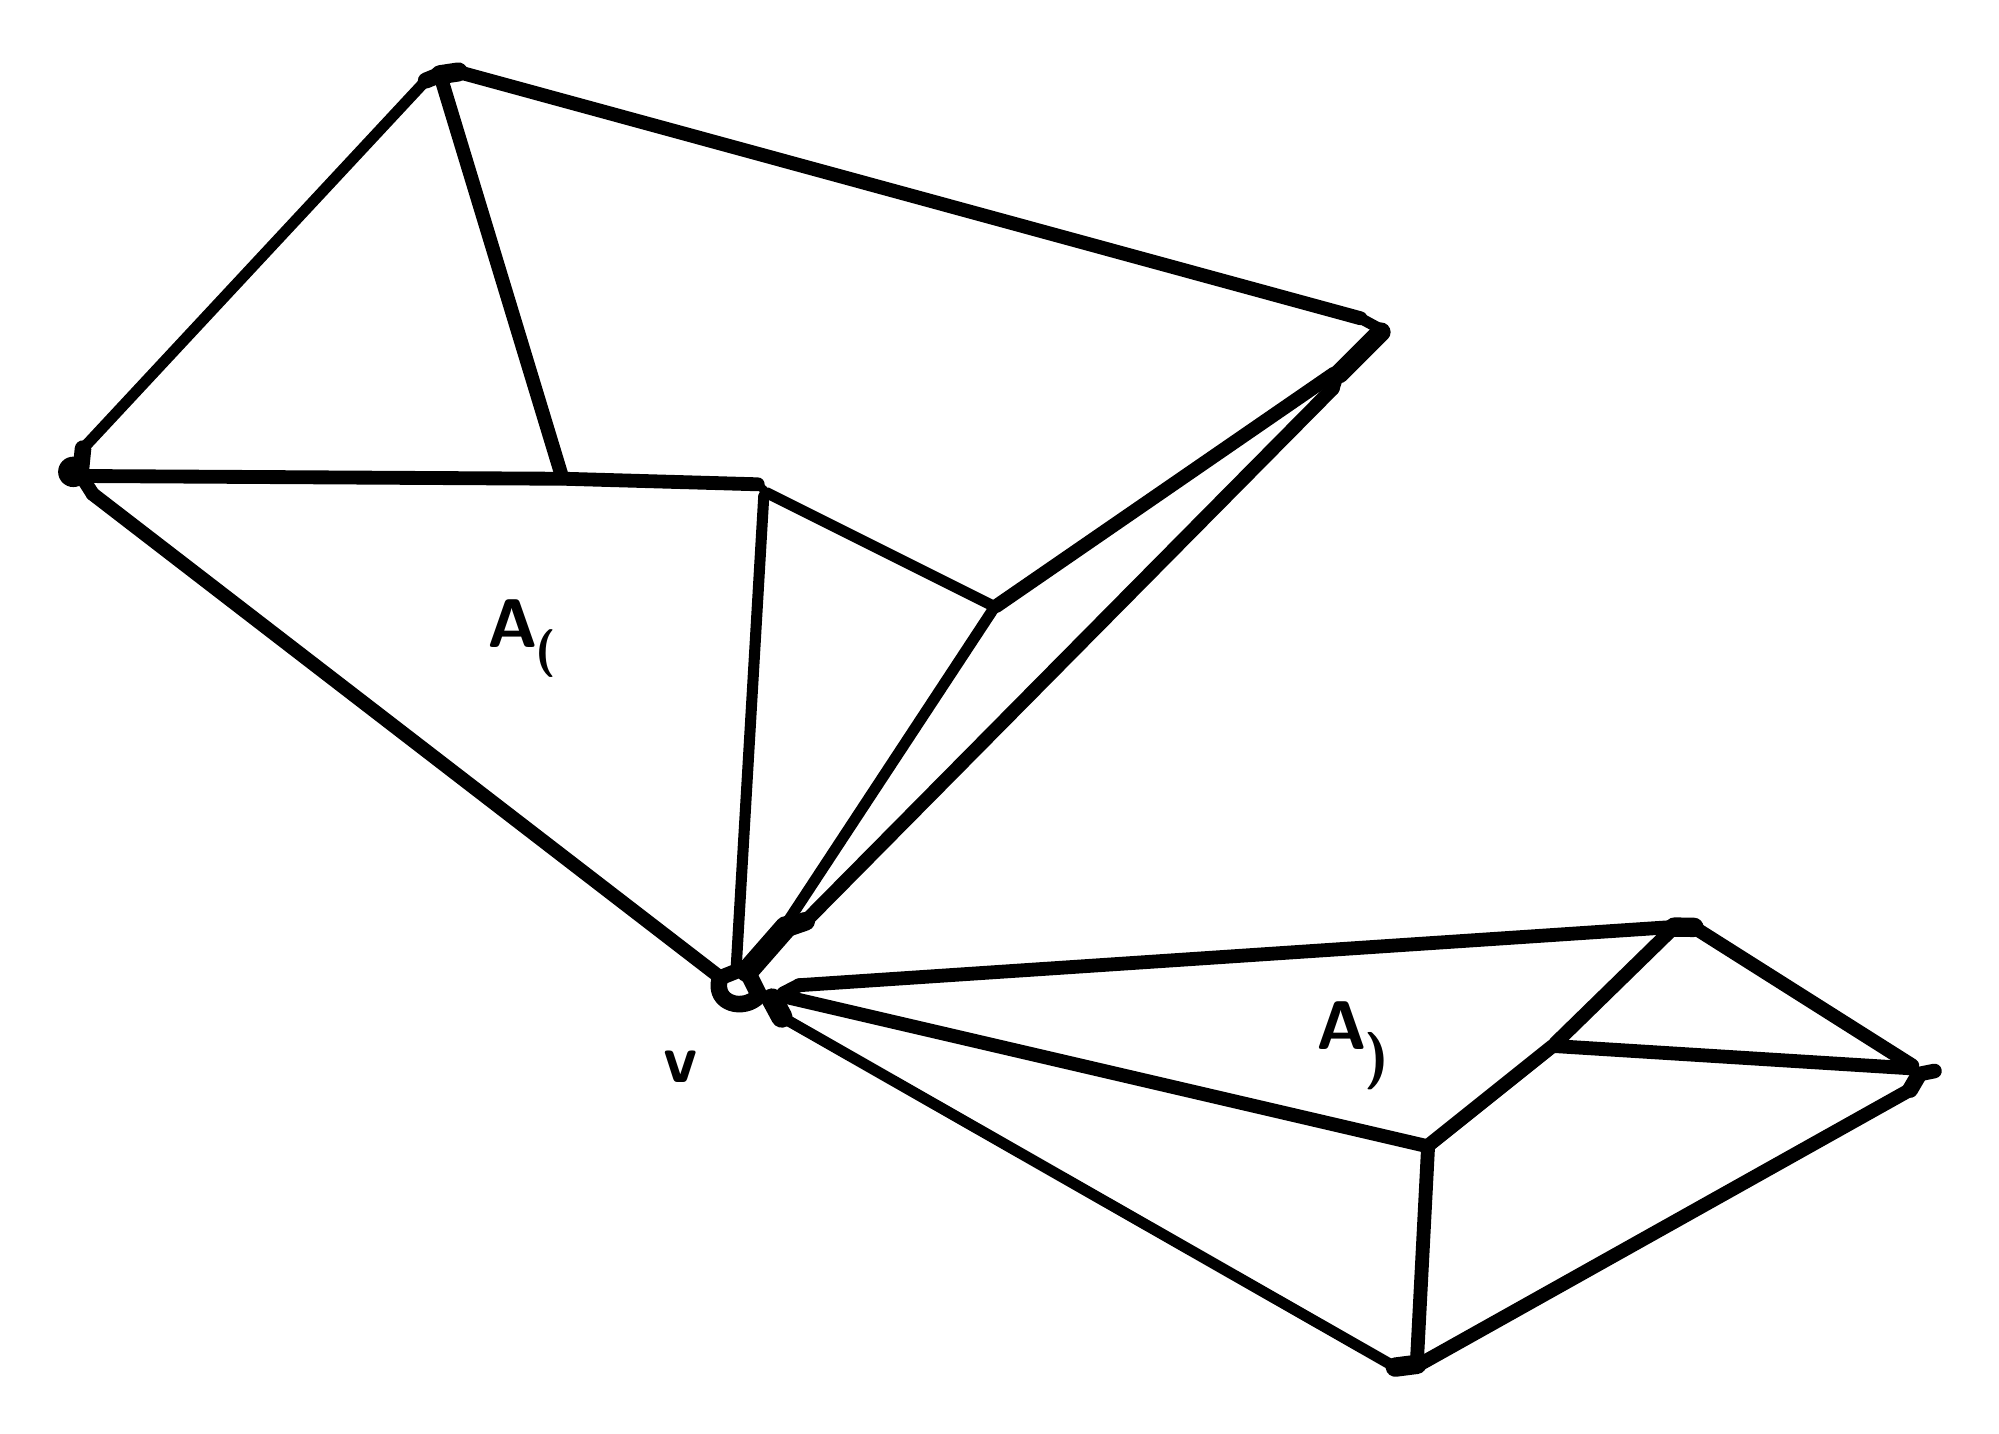
\begin{tikzpicture}[x=1pt, y=-1pt, line width=4.0pt, line cap=round, line join=round]

  %% ════ 填充区（prims2 的 fills）════

  %% ════ 直线段（prims2 的 strokes）════
  \draw[line width=4.0pt] (489.0,109.0) -- (481.6,105.0);
  \draw[line width=5.0pt] (481.6,105.0) -- (155.6,16.0);
  \draw[line width=6.9pt] (155.6,16.0) -- (149.0,17.0);
  \draw[line width=5.0pt] (594.0,326.0) -- (552.0,367.0);
  \draw[line width=7.0pt] (595.0,325.0) -- (602.1,325.1);
  \draw[line width=5.0pt] (602.1,325.1) -- (681.0,375.0);
  \draw[line width=5.0pt] (502.0,482.0) -- (506.0,405.0);
  \draw[line width=5.0pt] (250.0,343.0) -- (23.5,168.5);
  \draw[line width=5.0pt] (23.5,168.5) -- (20.0,163.0);
  \draw[line width=7.7pt] (269.0,351.0) -- (272.5,357.5);
  \draw[line width=4.0pt] (272.5,357.5) -- (494.2,484.0);
  \draw[line width=7.0pt] (494.2,484.0) -- (502.0,483.0);
  \draw[line width=5.0pt] (680.0,376.0) -- (552.0,368.0);
  \draw[line width=5.0pt] (350.0,209.0) -- (472.0,125.0);
  \draw[line width=5.5pt] (256.0,341.0) -- (251.0,343.0);
  \draw[line width=5.0pt] (194.0,163.0) -- (263.8,165.0);
  \draw[line width=3.0pt] (263.8,165.0) -- (266.0,167.0);
  \draw[line width=5.8pt] (149.0,17.0) -- (143.9,19.1);
  \draw[line width=4.0pt] (143.9,19.1) -- (20.0,152.1);
  \draw[line width=6.0pt] (20.0,152.1) -- (19.0,162.0);
  \draw[line width=5.0pt] (149.0,17.0) -- (193.0,162.0);
  \draw[line width=3.0pt] (268.0,350.0) -- (265.0,350.0);
  \draw[line width=8.0pt] (274.0,325.0) -- (260.0,341.0);
  \draw[line width=5.0pt] (273.0,350.0) -- (505.0,404.0);
  \draw[line width=4.9pt] (473.0,126.0) -- (471.6,130.4);
  \draw[line width=5.0pt] (471.6,130.4) -- (281.1,322.9);
  \draw[line width=6.8pt] (281.1,322.9) -- (275.0,325.0);
  \draw[line width=7.0pt] (489.0,110.0) -- (474.0,125.0);
  \draw[line width=5.0pt] (594.0,325.0) -- (278.8,346.0);
  \draw[line width=5.0pt] (278.8,346.0) -- (273.0,349.0);
  \draw[line width=4.0pt] (256.0,340.0) -- (266.0,169.0);
  \draw[line width=5.0pt] (506.0,404.0) -- (551.0,368.0);
  \draw[line width=4.0pt] (349.0,209.0) -- (267.0,168.0);
  \draw[line width=5.0pt] (503.0,483.0) -- (680.2,383.8);
  \draw[line width=5.8pt] (680.2,383.8) -- (683.0,379.0);
  \draw[line width=5.0pt] (193.0,163.0) -- (20.0,162.0);
  \draw[line width=5.3pt] (689.0,377.0) -- (684.0,378.0);
  \draw[line width=3.0pt] (257.0,341.0) -- (260.0,341.0);
  \draw[line width=6.0pt] (264.0,349.0) -- (260.0,341.0);
  \draw[line width=4.0pt] (274.0,324.0) -- (349.0,210.0);

  %% ════ 曲线（prims2 的 curves —— 三段式，坐标同为 (y,x)）════
  \draw[line width=6.0pt] (264.0,350.0) .. controls (258.8,355.4) and (247.9,352.9) .. (250.0,344.0);

  %% ════ 实心点 ════
  \fill (16.5,160.5) circle (5.5);

  %% ════ 标签（probe 直接给的 \node 行）════
  %% ⚠ 全部补了 fill=white：文字在最上层，否则与曲线交叉干扰
     \node[anchor=center,inner sep=0pt,fill=white,font=\fontsize{29.6}{37.0}\selectfont] at (175.2,215.5) {\textsf{\textbf{\textit{A}}}};   % box(163,204,19,22)
     \node[anchor=center,inner sep=0pt,fill=white,font=\fontsize{16.4}{20.5}\selectfont] at (187.3,226.3) {\textsf{\textbf{(}}};   % box(185,218,4,16)
     \node[anchor=center,inner sep=0pt,fill=white,font=\fontsize{30.3}{37.9}\selectfont] at (474.8,360.5) {\textsf{\textbf{\textit{A}}}};   % box(462,349,20,22)
     \node[anchor=center,inner sep=0pt,fill=white,font=\fontsize{21.5}{26.9}\selectfont] at (487.6,373.4) {\textsf{\textbf{)}}};   % box(484,362,5,22)
     \node[anchor=center,inner sep=0pt,fill=white,font=\fontsize{28.5}{35.6}\selectfont] at (236.2,375.4) {\textsf{\textbf{\textit{v}}}};   % box(228,366,14,16)

  % 钉死画布：否则超出的图元/控制点会把页面撑大，1:1 回比就失准
  \pgfresetboundingbox
  \path[use as bounding box] (0,0) rectangle (702,498);
\end{tikzpicture}
\end{document}

% ⚠ 待核清单（probe 拿不准，人眼过一遍）：
%   · 未识别/跳过：⑤ 跳过/未识别的字形
